
\titleformat{\chapter}
  {\gdef\chapterlabel{}
   \normalfont\sffamily\Huge\bfseries\scshape}
  {\gdef\chapterlabel{\thechapter\ }}{0pt}
  {
	\begin{tikzpicture}[remember picture,overlay]
	\node[yshift=-4cm] at (current page.north west)
	  {\begin{tikzpicture}[remember picture, overlay]
		\draw[fill=LightSkyBlue!20, draw=black, dashed] (0,0) rectangle
		  (\paperwidth,4cm);
		\node[anchor=east,xshift=.9\paperwidth,rectangle,
			  rounded corners=20pt,inner sep=11pt,draw,
			  fill=white, minimum width=6cm](name)
			  {  {\chapterlabel} \color{black}  #1   };
	   \end{tikzpicture}
	  };
   \end{tikzpicture}
   \vspace{2em}
  }




\usetikzlibrary{calc}
\title{
    \huge{\textcolor{blue}{Python股票分析}} \\ ~ \\
	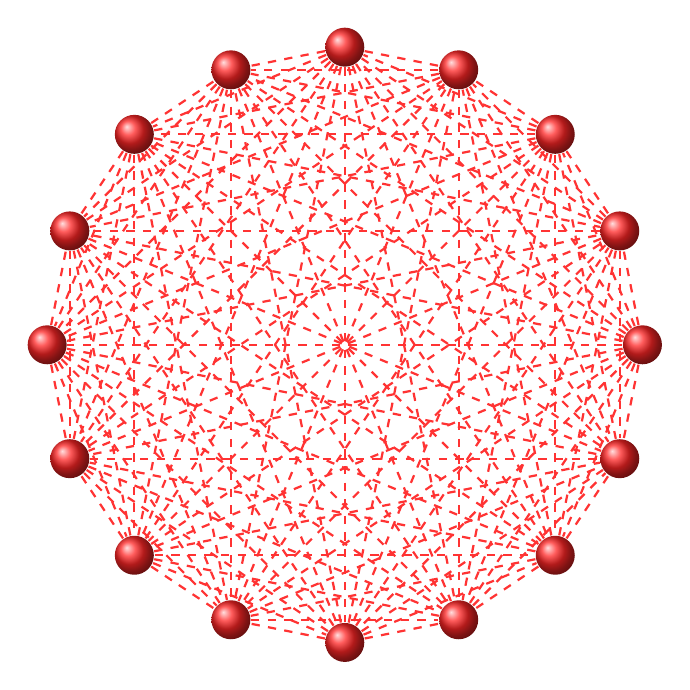
\begin{tikzpicture}[scale=0.7, transform shape,line width=0.2pt]
	  \foreach \x in {1,...,16}{%
		\pgfmathparse{(\x-1)*45+floor(\x/9)*22.5}
		\node[circle,inner sep=0.25cm,shading=ball, ball color=red!85] (N-\x) at (\pgfmathresult:5.4cm) [thick] {};
	  } 
	  \foreach \x [count=\xi from 1] in {2,...,16}{%
		\foreach \y in {\x,...,16}{%
		    \path (N-\xi) edge[-,draw=red!80, dashed, thick] (N-\y);
	  }
	}
	\end{tikzpicture}
}
\author{
	~\\
	~
}

% General definitions for all Chapters
%-------------------------------------------------------------------------------
% Define Page style for all chapters


% Set double spacing for the text
\doublespacing
%-------------------------------------------------------------------------------


% 1st page for the Title
%-------------------------------------------------------------------------------
\maketitle

%-------------------------------------------------------------------------------
%用于生成罗马计数的前言
\frontmatter


